\documentclass[12pt]{article}

\usepackage[margin=1in]{geometry}
\usepackage{fancyhdr}
\pagestyle{fancy}
\usepackage{amsmath}
\usepackage{amssymb}

% limit to particular location
\usepackage{float}

% graphics
\usepackage{graphicx}
% for subfigures
\usepackage{subcaption}

% better ref links
\usepackage{hyperref}

% adjust enum layout
\usepackage{enumitem}

% footnote in footer
\newcommand{\fancyfootnotetext}[2]{%
  \fancypagestyle{dingens}{%
    \fancyfoot[LO,RE]{\parbox{7cm}{\footnotemark[#1]\footnotesize #2}}%
  }%
  \thispagestyle{dingens}%
}

\lhead{HW4}
\chead{Digital Image Processing}
\rhead{B03902036}


\begin{document}

\section*{Problem 1}
Homework required one to design an algorithm to recognize the provided grayscale CAPTCHA based on provided training set.
Three separate stages can be deduced
\begin{enumerate}[itemsep=0px]
\item Training set feature extraction.
\item CAPTCHA character isolation.
\item Character recognition.
\end{enumerate}
In the following sections, I will walk through the trial-and-error process I had gone through.

\subsection*{Trial 1}
\subsubsection*{Training set feature extraction}
We are interested in the characters themselves, a mask with ones on the characters is closer to expectation. Trivial observation indicates no significant noise exists, and gray level is marginal to non-existence along character edges, we can try to threshold it directly by averaging global minimum and maximum. 
\begin{equation}
T = \sum_i \sum_j \frac{max(I(i, j))-min(I(i,j))}{2}
\end{equation}
Due to the fact that {\tt TrainingSet.raw} is provided as black-on-white style, thresholding criteria is reversed.
\begin{equation}
I(i, j) = 
\begin{cases}
	1, I(i, j) < T \\
	0, I(i, j) \geq T
\end{cases}
\end{equation}

\begin{figure}[H]
    \centering
    \begin{subfigure}[t]{0.5\textwidth}
        \centering
        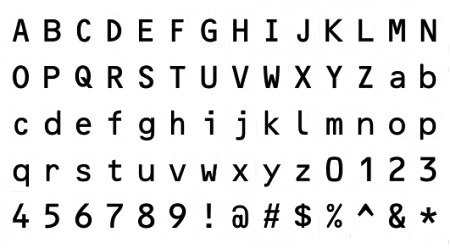
\includegraphics[height=1.5in]{images/training_original}
        \caption{Grayscale}
    \end{subfigure}%
    ~
    \begin{subfigure}[t]{0.5\textwidth}
        \centering
        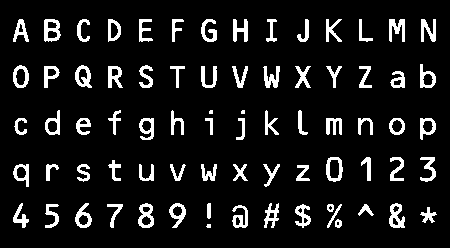
\includegraphics[height=1.5in]{images/training_binary}
        \caption{Binary}
    \end{subfigure}
    \caption{Pre-processed training set}
\end{figure}

The training set characters are displayed in montage, we need to isolate them to individual characters before proceeding to next step. The montage contains 14-by-5 characters, with consistence spacing between horizontal and vertical neighbors. We can easily calculate the appropriate spacing to separate them.
Margins of the image can causes misalignment after cropping, margin size of 5 and 7 pixels are empirically chose for horizontal and vertical edges respectively.

\begin{figure}[H]
    \centering
    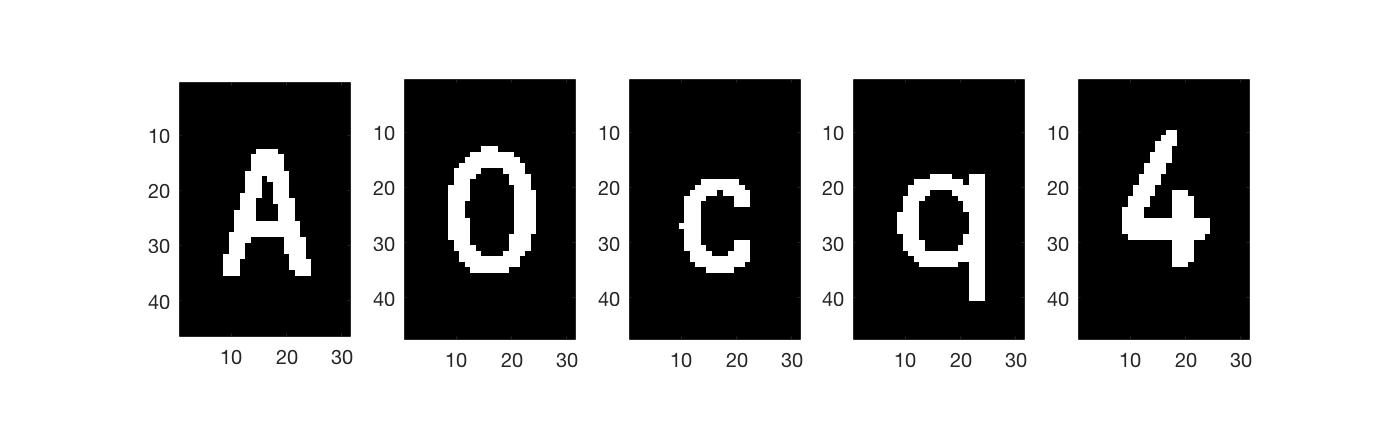
\includegraphics[width=0.7\textwidth]{images/training_cropped_col1}
    \caption{Cropped characters, first column is shown.}
\end{figure}

To perform further processing, I choose to resize them to image of size 32-by-32 pixels to ease the process.

\begin{figure}[H]
    \centering
    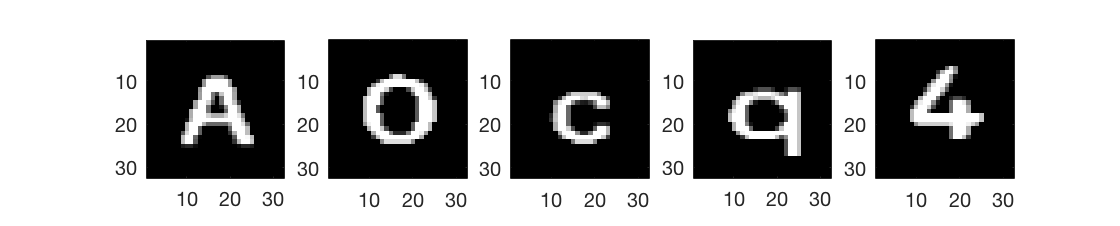
\includegraphics[width=0.7\textwidth]{images/training_resized_col1}
    \caption{Resized characters to square, first column is shown.}
\end{figure}

Characters seem to have enough differences from scanline perspective, therefore, I project sum each character along horizontal and vertical direction to derive their 2-by-32 feature vector in \autoref{fig:feature_direct_mip}.

\begin{figure}[H]
    \centering
    \begin{subfigure}[t]{0.5\textwidth}
        \centering
        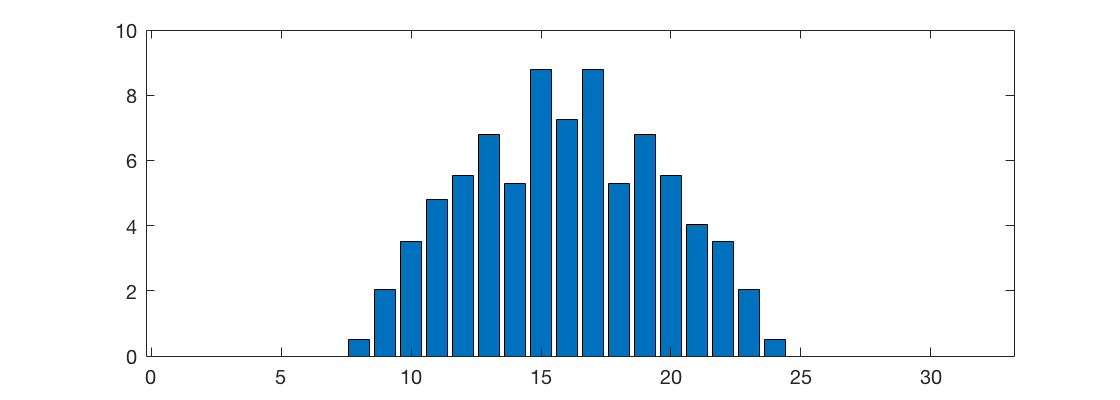
\includegraphics[height=1in]{images/feature_x_mip_a}
        \caption{X direction}
    \end{subfigure}%
    ~
    \begin{subfigure}[t]{0.5\textwidth}
        \centering
        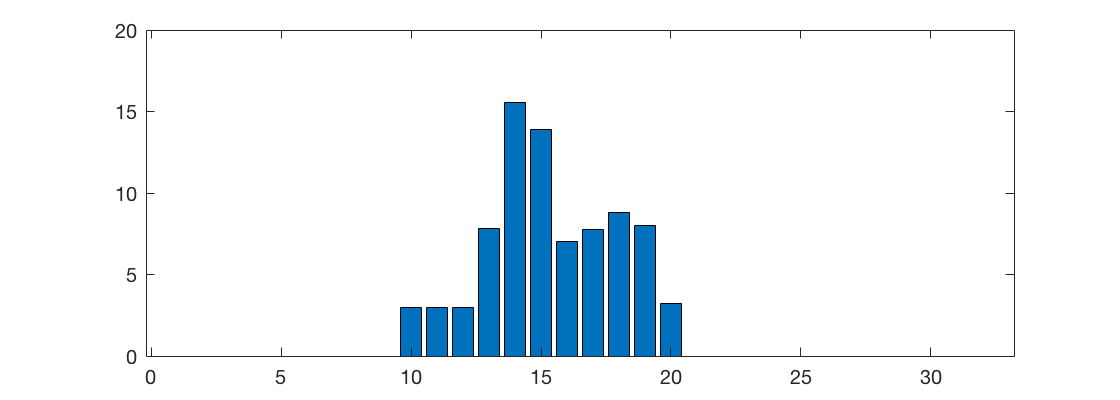
\includegraphics[height=1in]{images/feature_y_mip_a}
        \caption{Y direction}
    \end{subfigure}
    \caption{Cumulative sum projection of A}
    \label{fig:feature_direct_mip}
\end{figure}

\subsubsection*{CAPTCHA Character isolation}
Both sample images are easy to process as the training set. 

\begin{figure}[H]
    \centering
    \begin{subfigure}[t]{0.5\textwidth}
        \centering
        
\includegraphics[height=1in]{images/sample1_binary}
        \caption{Sample 1}
    \end{subfigure}%
    ~
    \begin{subfigure}[t]{0.5\textwidth}
        \centering
        
\includegraphics[height=1in]{images/sample2_binary}
        \caption{Sample 2}
        \label{fig:sample2_no_threshold}
    \end{subfigure}
    \caption{Binary sample images}
\end{figure}

Sadly, {\tt sample2.raw} contains unwanted speckle noises, visualized in \autoref{fig:sample2_no_threshold}. Therefore, median filter is applied specially for it. Kernel size of 3 is arbitrarily chosen by trials.

\begin{figure}[H]
    \centering
    \begin{subfigure}[t]{0.5\textwidth}
        \centering
        
\includegraphics[height=1in]{images/sample2_binary}
        \caption{Before}
    \end{subfigure}%
    ~
    \begin{subfigure}[t]{0.5\textwidth}
        \centering
        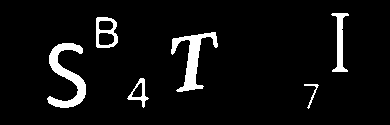
\includegraphics[height=1in]{images/sample2_binary_filtered}
        \caption{After}
    \end{subfigure}
    \caption{Median filter for {\tt sample2.raw}}
\end{figure}

For efficient labeling of connected components, disjoint-set algorithm based on handouts of Duke University {\it CS100e: Program Design and Analysis II} (\url{https://www2.cs.duke.edu/courses/cps100e/fall09/notes/UnionFind.pdf}) is used. However, characters such as {\tt i} will be labeled as separate components, hence, dilation is first performed prior to the labeling, and masked out dilated regions later on. Dilation kernel size is empirically chosen to be 7. 8-connected component is used.

\begin{figure}[H]
    \centering
    \begin{subfigure}[t]{0.5\textwidth}
        \centering
        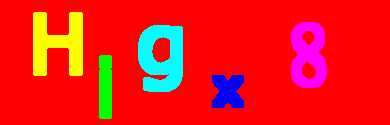
\includegraphics[height=1in]{images/sample1_labeled_dilated}
        \caption{Regions dilated}
    \end{subfigure}%
    ~
    \begin{subfigure}[t]{0.5\textwidth}
        \centering
        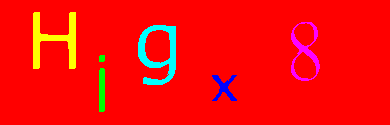
\includegraphics[height=1in]{images/sample1_labeled_masked}
        \caption{Masked result}
    \end{subfigure}
    \caption{Character labeling ({\tt sample1.raw})}
\end{figure}

Using labels, we can crop out each characters and sort them according to their horizontal position, implicit requirement for English reading convention.

\begin{figure}[H]
    \centering
    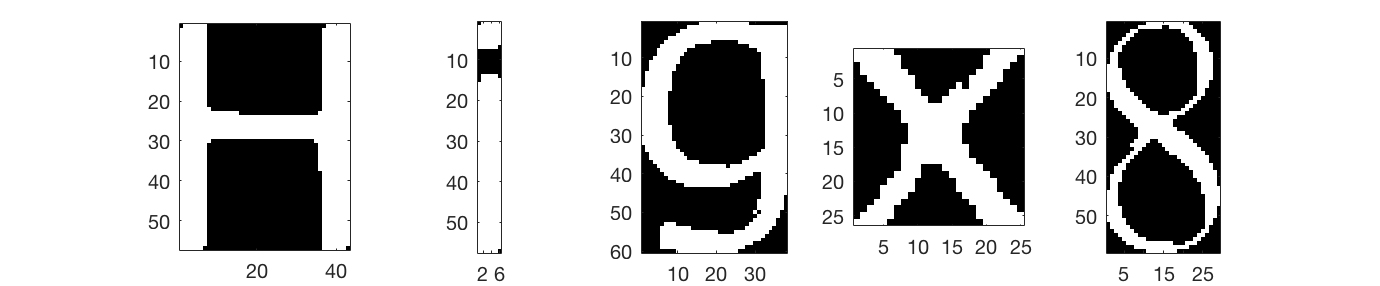
\includegraphics[width=0.7\textwidth]{images/sample1_cropped}
    \caption{Cropped characters}
\end{figure}

At last, characters are resized to 32-by-32 squares as well, same goes for {\tt sample2.raw}.

\begin{figure}[H]
    \centering
    \begin{subfigure}[t]{0.5\textwidth}
        \centering
        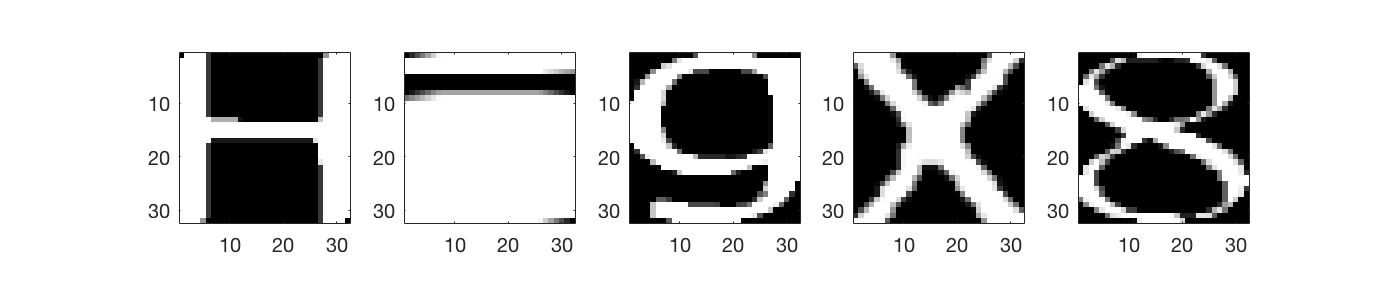
\includegraphics[width=\textwidth]{images/sample1_resized}
        \caption{{\tt sample1.raw}}
    \end{subfigure}%
    ~
    \begin{subfigure}[t]{0.5\textwidth}
        \centering
        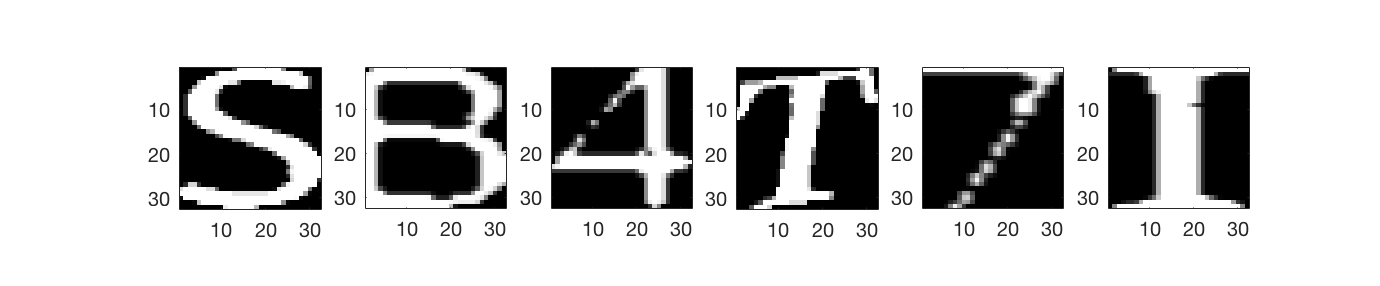
\includegraphics[width=\textwidth]{images/sample2_resized}
        \caption{{\tt sample2.raw}}
    \end{subfigure}
    \caption{Resized characters}
\end{figure}

\subsubsection*{Character recognition}
Directly subtract the differences between projection sum, I can retrieve the difference between curves, and use it as an index to find out which character is the most similar.

\begin{equation}
\begin{cases}
	d_x = \sum \vert \vec{c_x} - \vec{t_x} \vert^2 \\
	d_y = \sum \vert \vec{c_y} - \vec{t_y} \vert^2 \\
\end{cases}	
\end{equation}
where $\vec{c}$ is the feature character of CAPTCHA characters, while $\vec{t}$ is the feature character of training template. $d_x$ and $d_y$ are scalars. All the vectors are normalized prior to operations. A unified distance metric is used 
 \begin{equation}
 	d = \sqrt{d_x^2 + d_y^2}
 \end{equation}
 
\subsubsection*{Evaluation}
100\% error on both image.

\subsection*{Trial 2}
\subsubsection*{Training set feature extraction}
After reviewing the source code, I realize training set did not stretch the characters. Therefore 
\begin{figure}[H]
    \centering
    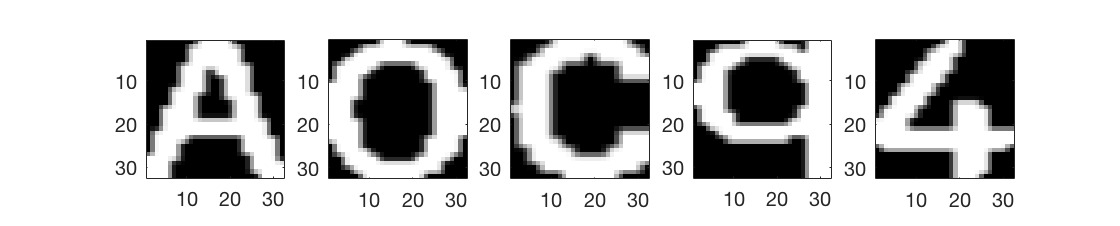
\includegraphics[width=0.7\textwidth]{images/training_resized2_col1}
    \caption{Stretched}
\end{figure}

\subsubsection*{Evaluation}
90\% average error rate. Only {\tt H} is correctly recognized in {\tt sample1.raw}. Apparently, direct curve comparison is not feasible. 

\subsection*{Trial 3}
\subsubsection*{Character recognition}
If we accumulate the projection result again, then the normalization to acquire the distance metric is essentially calculating the cumulative distribution function for pixel intensity along different direction (horizontal and vertical). By treating the problem as a binary classifier system, we can utilize the receiver operating characteristic (ROC) curve, but instead of favoring true positive direction, which requires maximizing the ROC curve area over $y=x$ line, we try to {\it minimize} that area, since same character should not deviate its distribution along any axis.

Feature vectors along both axis are now treated as sample points along X and Y direction, which are linearly interpolated to uniform X grid of size 32. The rationale of 32 is due to the resampled image size, applied earlier, is 32-by-32.

We can formulate the calculation of ROC area as 
\begin{equation}
	A_{ROC} = \sum \vert 
\end{equation}

\newpage
\newpage 

\subsection*{Boundary extraction}
\begin{figure}[H]
    \centering
    \begin{subfigure}[t]{0.6\textwidth}
        \centering
        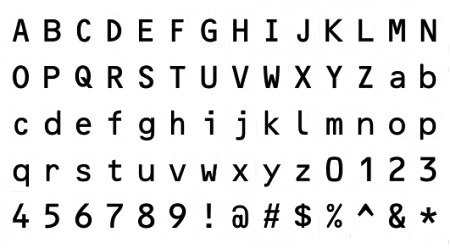
\includegraphics[height=1.5in]{images/training_original}
        \caption{Grayscale}
    \end{subfigure}%
    ~ 
    \begin{subfigure}[t]{0.24\textwidth}
        \centering
        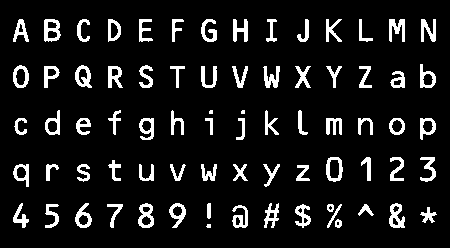
\includegraphics[height=1.5in]{images/training_binary}
        \caption{Binary}
    \end{subfigure}%
    ~
    \begin{subfigure}[t]{0.24\textwidth}
        \centering
        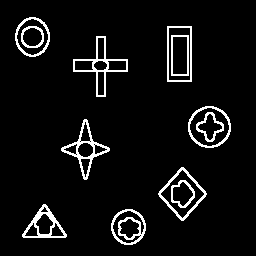
\includegraphics[height=1.5in]{images/B_m5}
        \caption{$5 \times 5$}
    \end{subfigure}%
    ~
    \begin{subfigure}[t]{0.24\textwidth}
        \centering
        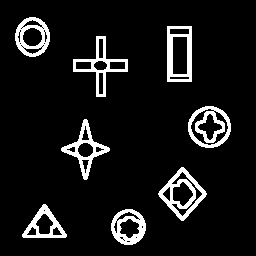
\includegraphics[height=1.5in]{images/B_m7}
        \caption{$7 \times 7$}
    \end{subfigure}
    \caption{$B$}
\end{figure}
Boundary extraction is composed of erosion and its complement
\begin{equation}
	B = I_1 \wedge \sim (I_1 \ominus SE)
\end{equation}
where $SE$ is the structural element, square in this case.
When the sides of $SE$ increases, the more the erosion is applied on $I_1$, causing more blanked region appeared after $\& ~(I_1 \ominus SE)$, leading to thicker edges.

\subsection*{Skeletonizing}
\begin{figure}[H]
    \centering
    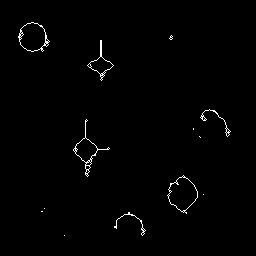
\includegraphics[height=2.5in]{images/S}
    \caption{$S$, skeletonized $I_1$}
\end{figure}
The implementation try to follow the implementation from textbook, which requires two set of lookup tables. General operation is 
\begin{equation}
	G = X \cap \lbrack \sim M \cup P \rbrack
\end{equation}
where $X$ is the input image, $G$ is the output image, $M$ is the conditional marker determined in the process, and $P$ is the inhibiting variable.

During the first pass, $M$ is determined by hit-and-miss transformation using the kernel from \autoref{tbl:conditional}. 
I put tons of time to figure out the decimal equivalent of them, I might as well put my result here, and there seems to be no one posting this out there on the Net.
\begin{table}[H]
\caption{Conditional}
	\centering
	\begin{tabular}{c|c}	
	Type & Decimal number \\
	\hline
	\hline
	S1 & 64, 16, 4, 1\\
	S2 & 128, 32, 8, 2\\
	S3 & 192, 96, 48, 24, 12, 6, 3, 129 \\
	TK4 & 160, 40, 10, 130 \\
	STK4 & 193, 112, 28, 7 \\
	ST5 & 176, 161, 104, 194, 224, 56, 14 ,131 \\
	ST6 & 177, 108 \\
	STK6 & 240, 225, 120, 60, 15, 135, 195 \\
	STK7 & 241, 124, 31, 199\\
	STK8 & 227, 248, 62, 143\\
	STK9 & 243, 231, 252, 249, 124, 63, 159, 207\\
	STK10 & 247, 253, 127, 223\\
	K11 & 251, 254, 191, 239\\
	\end{tabular}
	\label{tbl:conditional}
\end{table}

During the second pass, which is coined as the unconditional stage, output result is determined by combination of $X$ and $M$. 
Since there are spaces for combinations in the textbook kernel list, I separated them to three categories to ease the computation process.

\paragraph{First} type is simply equal-or-not comparison with values from \autoref{tbl:unconditional_eq}. One simply extract the surrounding pixels 
\begin{equation}
	V = \sum_{i\in\text{neighbors}}{M_i 2^i}
\end{equation}
where $V$ is the corresponding decimal value constructed by the fully connected neighbors.
Most significant bit is the first pixel, designated $M_0$ in the textbook.

\begin{table}[H]
\caption{Unconditional, EQ}
	\centering
	\begin{tabular}{c|c}	
	Type & Decimal number \\
	\hline
	\hline
	Spur & 1, 4, 64, 16\\
	4-connected & 2, 128, 8, 32\\
	L & 160, 40, 130, 10
	\end{tabular}
	\label{tbl:unconditional_eq}
\end{table}

\paragraph{Second} type requires one to provide a mask before comparison.
The comparison is composed of two parts
\begin{equation}
\begin{cases}
	P_1 = (X \vee K_M) \wedge K_C \\
	P_2 = (T \wedge \sim K_M) \wedge (K_C \wedge \sim K_M)\\
\end{cases}
\label{eq:unconditional_or_eq_eq}
\end{equation}
and the final result is determined by 
\begin{equation}
	P = P_1 \wedge P_2
\end{equation}
$P_1$ used the mask to ignore flexible $D$ terms in the table provided in the textbook, while $P_2$ verifies the constant terms, $M$, $0$ and $1$ are satisfied as well.
$K_M$ is the mask while $K_C$ is the conditional equivalent decimal number, both of them are enlisted as a pair $(K_M, K_C)$ in \autoref{tbl:unconditional_or_eq}.

\begin{table}[H]
\caption{Unconditional, OR-EQ}
	\centering
	\begin{tabular}{c|c}	
	Type & (Mask, Condition) \\
	\hline
	\hline
	Corner & (31, 255), (241, 255), (199, 255), (124, 255) \\
	Tee & (84, 252), (213, 255), (117, 255), (93, 255) \\
	Diagonal & (17, 181), (68, 109), (17, 91), (68, 214)\\
	\end{tabular}
	\label{tbl:unconditional_or_eq}
\end{table}

\paragraph{Third} type is similar to the second type, but instead of equivalent, it requires unequal, since in the textbook, 
\begin{equation}
	A \cup B \cup C = 1
\end{equation}
in other words, one of them has to be 1, complementary is relatively easy to test for.

Under this consensus, \autoref{eq:unconditional_or_eq_eq} can be modified as
\begin{equation}
\begin{cases}
	P_1 = \sim ((X \vee K_M) \vee K_C) \\
	P_2 = (T \wedge \sim K_M) \wedge (K_C \wedge \sim K_M)\\
\end{cases}
\label{eq:unconditional_or_eq_eq}
\end{equation}

\begin{table}[H]
\caption{Unconditional, OR-NEQ}
	\centering
	\begin{tabular}{c|c}	
	Type & (Mask, Condition) \\
	\hline
	\hline
	Vee & (184, 248), (42, 62), (138, 143), (162, 227) \\
	\end{tabular}
\end{table}

If short segments are unwanted, pruning algorithm can be employed. In my implementation, some objects seem to being thinned too aggressively, however, I haven't found the pitfalls in the pipeline for the time being. 

\section*{Problem 2}
\subsection*{Law's method}
\begin{figure}[H]
    \centering
    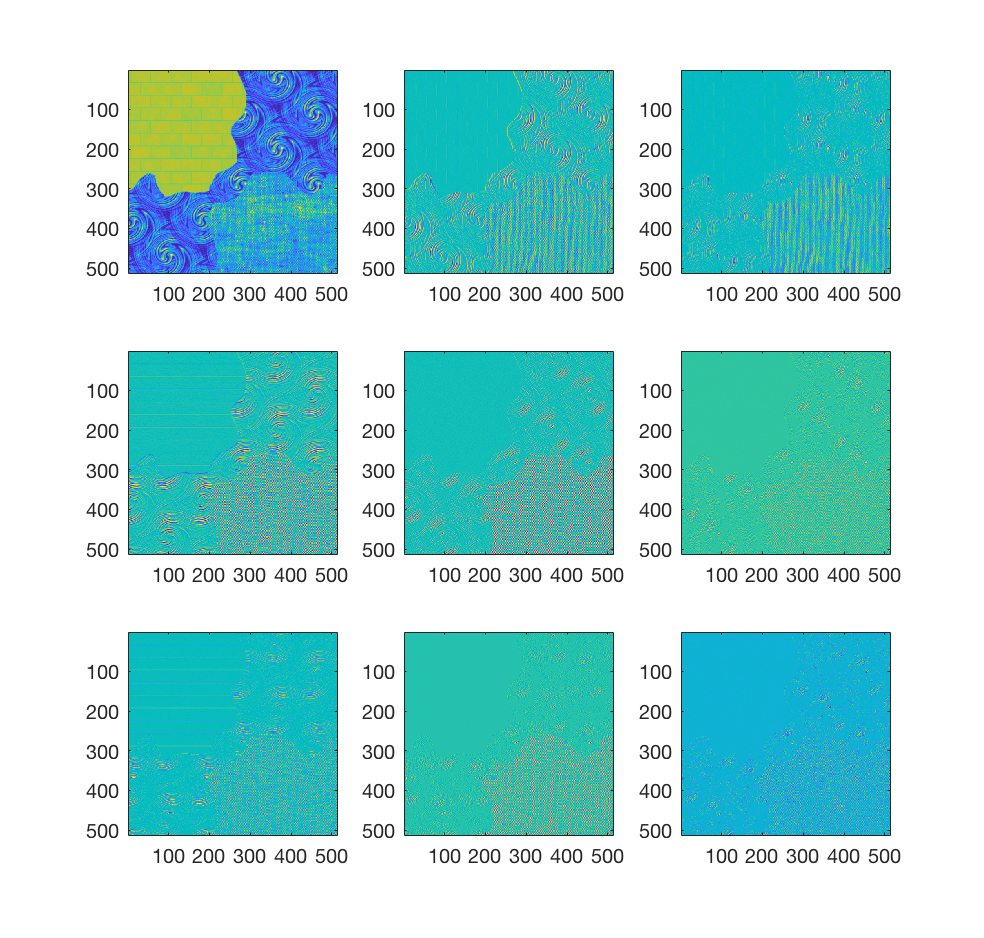
\includegraphics[height=5in]{images/M}
    \caption{Filters}
    \label{fig:law_filters}
\end{figure}
\autoref{fig:law_filters} shows the results after applying 3-by-3 filters described in the slides, oriented from left-to-right, top-to-bottom are low-to-high pass.

The result is not quite clear in this case, however, the simple energy function of windows size 15,
\begin{equation}
	T = \cap \cap_{(i, j) \in w} M(i, j)^2
\end{equation}
yields fabulous result.

\begin{figure}[H]
    \centering
    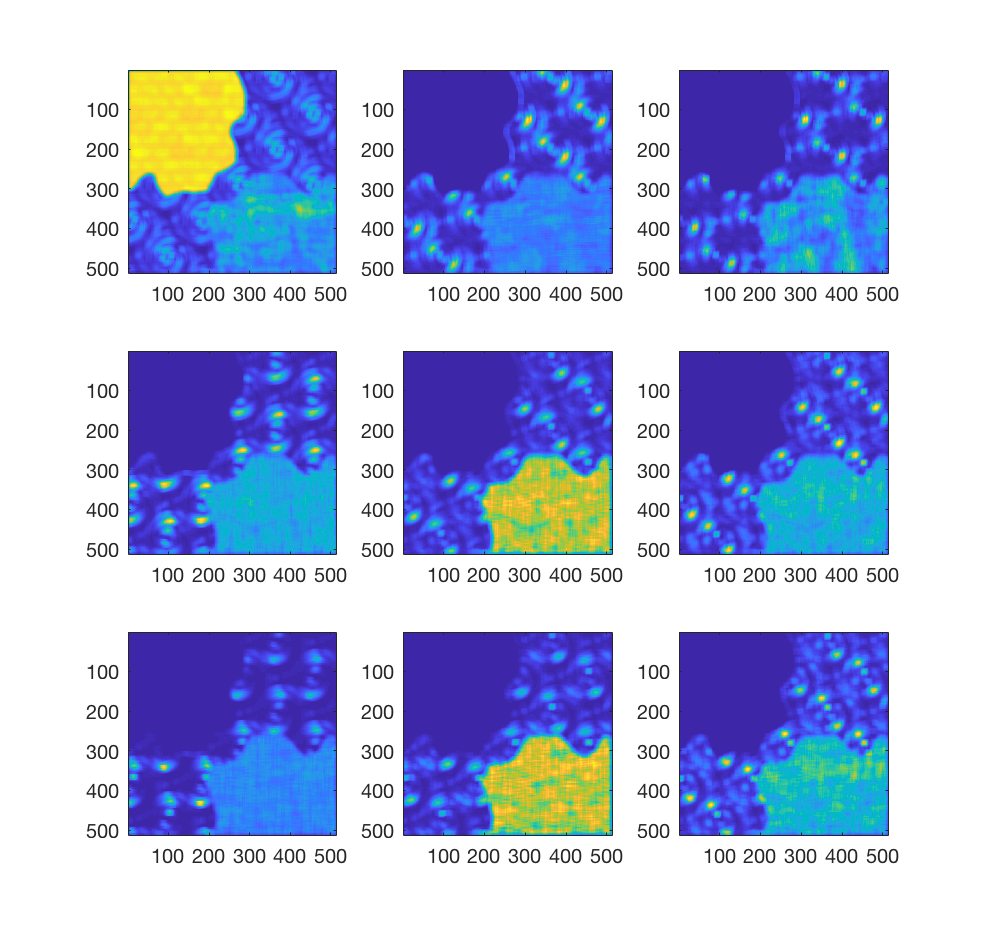
\includegraphics[height=5in]{images/T}
    \caption{Energy}
    \label{fig:law_energy}
\end{figure}
\autoref{fig:law_energy} oriented the same way as \autoref{fig:law_filters}, in this case, we can easily see the whirls have their frequency components evenly distributed, while the cloth on the lower right is relatively high frequency, compares to the brick wall on the upper left side.

Using classic K-mean clustering algorithm with three classes and randomly initialized seeds, results in acceptable result.

\begin{figure}[H]
    \centering
    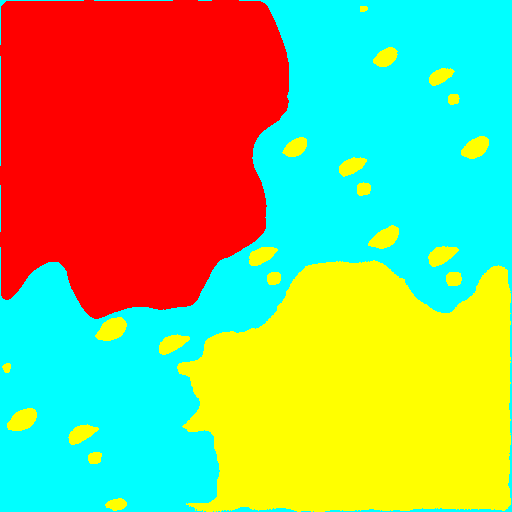
\includegraphics[height=2.5in]{images/K}
    \caption{Segmented reuslt}
    \label{fig:kmean}
\end{figure}

However, blobs can be observed in the middle section of the whirls, one may remove them by removing objects smaller then specified size.

\subsection*{Texture swapping}
Efos-Leung algorithm is adapted for this task, courtesy to the MATLAB implementation presented by {\it asteroidhouse} on GitHub, with small modification, one can adapt the algorithm for partial texture synthesis (patch the regions, relatively smaller), instead of full synthesis (generate entire image from a small patch). 

The algorithm generates the texture pixel-wise, outwards from the initial seed, using pixels inside a defined windows as the context. 
The basic idea is modeling the patch as a generalized Markov chain, similar to the $n$-gram idea in natural language processing. 
Therefore, one build a probability for tables for each $n$-gram pixel combinations through repeatedly sample in the window, and synthesize new pixels by observing the most probable intensity in the sampled $n$-gram "corpus".

\begin{figure}[H]
    \centering
    \begin{subfigure}[t]{0.3\textwidth}
        \centering
        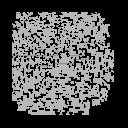
\includegraphics[height=2in]{images/tex1}
        \caption{Class 1}
        \label{fig:synth_1}
    \end{subfigure}%
    ~ 
    \begin{subfigure}[t]{0.3\textwidth}
        \centering
        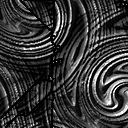
\includegraphics[height=2in]{images/tex2}
        \caption{Class 2}
        \label{fig:synth_2}
    \end{subfigure}%
    ~
    \begin{subfigure}[t]{0.3\textwidth}
        \centering
        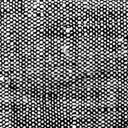
\includegraphics[height=2in]{images/tex3}
        \caption{Class 3}
        \label{fig:synth_3}
    \end{subfigure}%
    \caption{Synthesized}
    \label{fig:synth}
\end{figure}

Using random patch size pick in the regions, no larger than 128-by-128, due to deadline, window size is configured to 4, and synthesis result size is restricted to 128-by-128 instead of full size 512-by-512. 
\autoref{fig:synth} shows the synthesized result of three identified categories retrieved from previous section.
Synthesis iteration is limited to 1000 due to limited time as well, instead of ensuring all the pixels are determined.

As one may expected, insufficient window size will result in information lost, causing the texture unable to be continuous, visualized as the crack in \autoref{fig:synth_2}.
The brick pattern requires much larger window to capture the grid lines, this will significantly increase the synthesis time, very limited window and limited iteration cycle not only lead to incomplete output, but also incorrect pattern in \autoref{fig:synth_1}. 

For pattern that has high frequency components, visualized in \autoref{fig:law_energy}, relatively small window and less iteration is required as hypothesized, the result in \autoref{fig:synth_3} is pleasing as well.


Unable to generate complete synthesized swapped image on time.

\end{document}
              